\chapter{卖出看跌期权\label{CH19}}
相对于卖出备兑看跌期权,卖出未备兑看跌期权的情形更为常见。因此,我们首先介绍卖出未备兑看跌期权。这是一个看多的策略。
\section{卖出未备兑看跌期权}
卖出无备兑看跌期权的策略在许多方面都和卖出备兑看涨期权的策略相像。你可以注意到它们的盈利图的形状相同,这就是说这两个策略是相等的。

\begin{figure}
    \centering
    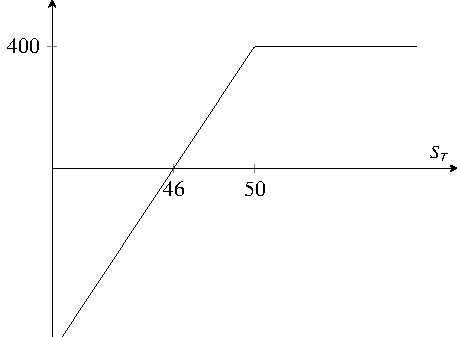
\includegraphics[width=0.8\textwidth]{IMG/Uncovered sale of a put.pdf}
    \caption{卖出无备兑看跌期权}
    \label{fig:uncovered put short}
\end{figure}

交易者在两个策略中对标的股票都是看多的,或者至少是中性的。如果标的股票向上运动,未备兑看跌期权的卖出者就有盈利,也许是收入的全部权利金。如果标的股票在到期日没有变化(中性),看跌期权的卖出者在最初卖出这个期权时所收入的全部权利金就变成了他的盈利。如果这手看跌期权是虚值的,这就代表了他的最大盈利,因为这就意味着整个看跌期权的权利金都是由时间价值组成的。不过,对一手实值看跌期权来说,时间价值只是整个期权权利金中的一部分。

在这两种策略中,如果头寸建立的时候股票价格高于期权行权价,那么,实现最大盈利的概率就更大。这代表了不是那么激进的运用:开始时卖出虚值看跌期权,它同卖出实值备兑看涨期权是相等的。

\textbf{更为激进的使用卖出裸看跌期权的方法是一开始就卖出实值看跌期权。}实值看跌期权的卖出者在开始时就可以收到较大数量的权利金,如果标的股票上涨得足够高,他可以得到一大笔盈利。使用这种方法增加了潜在盈利,因此也承担了更大的风险。如果标的股票下跌,实值看跌期权的卖出者亏钱的速度会比一开始卖出虚值看跌期权的情形更快。

要总结这些并不难,只需要注意到,无论是在卖出裸看跌期权策略中还是在卖出备兑看涨期权的策略中,在股票高于卖出的期权的行权价时建立起来的头寸都是不那么激进的头寸。如果股票价格一开始就低于期权的行权价,那么,由此建立的头寸就是较为激进的头寸。
\section{后续行动}
如果标的股票价格下跌,裸看跌期权的卖出者就应当采取保护性的后续行动。最简单的后续行动就是如果股票下跌,就承担少量亏损,将头寸平仓。由于实值看跌期权往往会很快失去时间价值,如果股票朝对他不利的方向运动,他会发现他的亏损常常相当小。

在卖出备兑看涨期权策略里,我们曾建议策略家应当在可能的情况下尽量向下挪仓。这样做而不是将备兑看涨期权头寸平仓的理由之一是平仓手续费会很大,一般来说你不可能老是买入、卖出股票。更有利的做法是保留股票头寸,只是将看涨期权向下挪仓。在卖出裸看跌期权中不存在这样的手续费劣势。当交易者选择了裸看跌期权头寸时,他只是买回看跌期权。因此,对裸看跌期权卖出者来说,向下挪仓就不是那么有利。
\section{对卖出裸看跌期权进行评价}
在选择卖出看跌期权时,必须有一个起码的可以接受的收益水平。例如,交易者可以决定,为了选这个头寸来进行最大的下行方向的保护,这个头寸必须至少提供 12\% 的年收益率。有了这样的要求,就可以排除掉上面所说的极端情况。一旦经过这样的审视,就可以用正常的方式来对各种选择进行排序。收益最高的卖出看跌期权应当是较为激进名单的首选,在下行方向提供最高百分比保护的则应当成为较为保守的名单的首选。在最为严谨的意义上,应当正确地使用一个将标的股票的波动率结合在内的更为高级的技巧。
\section{按低于市价买入股票}
\begin{tcolorbox}
    XYZ 是一只价值 60 美元的股票,投资者觉得如果在 55 的价格上就值得买入。他在市场上放了一个限价 55 的公开买入指令。3 个月之后,XYZ 的价格下跌到 57,但没有跌得更低。之后它反转方向,大幅度上涨,于是限价买入指令从来没有被启动过,投资者失去了这次机会。
\end{tcolorbox}
这个假想的投资者可以使用一手裸看跌期权来为他服务。假定当 XYZ 最初在 60 的时候,这个投资者不是放置一个公开限价指令,而是卖出一手 3 个月的裸看跌期权,价格为 5 点。这样,只要 XYZ 在到期时价格低于 60,他就可以按 60 的价格买入股票。也就是说,他必须为这个股票付 60 的价格。但由于他在卖出看跌期权时已经收到了 5 点,他的净成本就是 55。因此,即使 XYZ 在到期日的价格为 57,而且从来没有低于过这个价格,这个投资者仍然可以 55 的成本买到 XYZ。

当然,如果 XYZ 立刻上涨,而且在到期日时价格高于 60,这个看跌期权就不会被指派,投资者也不能持有 XYZ。不过,他仍然能从卖出看跌期权中得到 500 美元,看跌期权现在没有任何价值了。因此,由于采取了行动而不只是等待,看跌期权的卖出者在他的投资中起了更为积极的作用。他至少为他的努力得到了某种收益,即使他没有能够买到股票。

这个技巧对许多最终想要持有股票的投资者都有用处。大规模投资组合的管理者和个体投资者都可以发现以这个目的卖出看跌期权是一种有用的策略。这是一种试图按比目前市场价格更低的价格来积累股票头寸的方法。如果股票价格上涨,没有能够买到股票,那么,投资者至少有看跌期权权利金收入来弥补他的努力。

\paragraph{必须小心} 尽管卖出裸看跌期权看上去似乎性质温和,由于以下的两个原因,它有可能是非常危险的:(1)如果标的股票暴跌,就有可能出现巨额的亏损;(2)因为质押要求相当低,所以有高度的杠杆效应。如果你“不在乎持有”一只“高质量”的股票,那么,就它卖出虚值看跌期权,听上去是个不错的主意。但是,任何股票都有可能出现灾难性的暴跌。
\section{卖出备兑看跌期权}
按照定义,当投资者还相应持有一手看跌期权,其行权价等于或高于其卖出的看跌期权时,其卖出的看跌期权才是备兑的。这是一个价差。不过,就保证金的目的而言,如果投资者在卖出一手看跌期权的同时也在卖空标的股票,他就是备兑的。保证金的要求是针对卖空股票的,在卖空看跌期权方面没有这样的要求。这样就构造了一个潜在盈利有限的头寸,如果标的股票的价格在到期日时低于看跌期权的行权价,就能实现这个盈利。在上行方向有无限的风险,因为如果标的股票价格上涨,卖空股票的一侧就会积累亏损,而卖出看跌期权一侧的盈利是有限的。这事实上是与卖出裸看涨期权相等的头寸,不同的只是备兑看跌期权卖出者必须就标的股票支付股息,如果有这样的股息存在的话。\textbf{卖出无备兑看涨期权比起这个策略有一个好处:它的手续费要低得多。此外,看涨期权的时间价值一般比看跌期权要高,因此,裸看涨期权卖出者能得到更多的时间价值。卖出备兑看跌期权是一个很少有人使用的策略,它不如卖出裸看涨期权。}
\section{卖出看跌期权比率}